% Created 2021-03-04 周四 11:46
% Intended LaTeX compiler: pdflatex
\documentclass[11pt]{article}
\usepackage[utf8]{inputenc}
\usepackage[T1]{fontenc}
\usepackage{graphicx}
\usepackage{grffile}
\usepackage{longtable}
\usepackage{wrapfig}
\usepackage{rotating}
\usepackage[normalem]{ulem}
\usepackage{amsmath}
\usepackage{textcomp}
\usepackage{amssymb}
\usepackage{capt-of}
\usepackage{hyperref}
\date{\today}
\title{}
\hypersetup{
 pdfauthor={},
 pdftitle={},
 pdfkeywords={},
 pdfsubject={},
 pdfcreator={Emacs 27.1 (Org mode 9.4.4)}, 
 pdflang={English}}
\begin{document}

\tableofcontents

---
title: "理解动态规划与warshall算法"
date: 2021-02-19T13:35:34+08:00
draft: false
tags: ['algorithm', 'math']
categories: ['learning']
cover: '/img/2021-02-19\textsubscript{dijkstra.jpg}'
---
今天刚好在离散里学了用来计算传递闭包的warshall算法,就在这里把离散里计算闭包的算法
和动态规划一起整理一下。
\section{集合、关系和闭包}
\label{sec:org7981eda}
要理解闭包首先需要了解集合和关系(函数)。
在离散数学中我们讨论的集合都是非公理化的朴素集合论(会导致罗素悖论)。有时间可以了解下公理集合论。
\subsection{关系与函数}
\label{sec:org111e7d9}
关系: 关系是一个集合中的元素到另一个集合中元素的映射方式。二元关系是两个集合笛卡尔积的子集。
关系能够具有的性质包括自反性,对称性,传递性,反自反性,反对称性。具有自反、堆成、传递性
的关系称为等价关系。其他的特殊关系有偏序(包含全序、良序、字典序)

函数:函数可以看作一种特殊的关系。
函数是每个定义域中元素到唯一一个值域中元素的映射.

A function from A to B is an assignment of exactly one element
of B to each element of A.

\href{https://www.shuxuele.com/sets/injective-surjective-bijective.html}{函数的种类}包括
\begin{itemize}
\item 单射 一一对应(one-to-one)函数:如果定义域中的两个元素不相等,那值域中对应的两个元素也肯定不相等.
\item 满射(onto)函数:值域中每个值都有对应的定义域元素.
\item 双射: 满足单射及满射
\end{itemize}
\subsection{闭包}
\label{sec:org9db1458}
闭包:一个集合具有某个性质的最小超集。例如在一个集合S上关系R的自反闭包是R并S0, S0是集合S中所有元素到自身关系的集合。
其他常用的闭包还有对称闭包和传递闭包。自反闭包记作r(R),对称闭包s(R),传递闭包t(R).

一个关系的自反闭包与对称闭包计算都很简单,传递闭包要麻烦些。一个具有传递性的关系是指在该关系中,
如果出现了(a,b)和(b,c),则(a,c)也存在。想得到一个关系具有传递性的最小超集,我们要检查当前该关系中所有满足(a,b) (b,c)
的pair,得到(a,c)后加入。但是只进行一次后不一定能得到我们想要的传递性关系。比如原先关系R为\{(a,b), (b,c), (c,d)\},
进行一次计算后得到的R1是\{(a,b), (b,c), (c,d), (a,c), (b,d)\}。R1中存在(a,b)和(b,d),但是没有(a,d),并不是我们想要的
自反闭包。我们需要再做一次相同的步骤。在一个无穷关系中,相同的步骤需要执行无穷次。这就是计算传递闭包的算法。

我们把算法整理一下写出来是这样的
\begin{center}
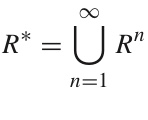
\includegraphics[width=.9\linewidth]{c:/img/2021-02-20_transitive-closure.png}
\end{center}

在有限关系中,相同的步骤最多只需要执行n次。n为集合中元素的个数。该定理证明需要引入路径path的概念。我们把从一个元素a通过一系列
传递关系最终到达另一元素b中间这一系列关系称为a到b的路径。经过关系的数量称为路径长度。可以证明,集合中任意两点间路径长度最长为n。
因为若有一条路径长度>n,其中必定经过某一顶点大于一次,形成环路。将该环路去掉可以得到长度<=n的路径。易证R\textsuperscript{i是集合中有长度为i的}
路径的连接矩阵(如果a到b间有一条长度为i的路径,R\textsuperscript{i}[a,b]=1,否则R\textsuperscript{i}[a,b]=0)。这样我们可以在有限的步骤(n步)得到有限集合的
传递闭包。


可以用伪代码表示
\begin{verbatim}
procedure transitive closure
A := M
B := A
for i:= 2 to n
  A := A * M   // 计算A^i
  B := B or A
return B
\end{verbatim}
该算法每次计算 A := A*M  的复杂度为O(n\textsuperscript{3}), B := B or A 复杂度为O(n\textsuperscript{2})。算法整体复杂度为O(n\textsuperscript{4})。

\section{floyd-warshall算法}
\label{sec:org07d6980}
关于dijkstra算法与floyd算法的介绍我找到了一篇介绍\href{https://www.cnblogs.com/biyeymyhjob/archive/2012/07/31/2615833.html}{博客}。

warshall算法是一种可以用更低复杂度计算传递闭包的算法。之前我们得到的算法计算了n次A\textsuperscript{i}, 每次矩阵乘法复杂度为O(n\textsuperscript{3}). warshall算法提供了一种
O(n\textsuperscript{3})的方法得到最终的传递闭包。

如果点i与点j间有一点k,可以找到关系(i,k), (k,j),我们就将(i,j)看作可用长度为n的路径连接,加入当前矩阵。我们检测n次得到最终的长度0-n的路径
矩阵。每次把一点作为k,检查所有i与j,复杂度为O(n\textsuperscript{2})。最终得到的算法复杂度为O(n\textsuperscript{3}).

\section{动态规划}
\label{sec:org381c759}
\subsection{分治法}
\label{sec:org0d5d661}
分治法的核心思想是将问题划分为独立的子问题,递归求解后合并得到问题的解。典型的例子有归并排序。
归并排序的步骤:1. 拆分 2. 递归求解 3. 归并 
\subsection{动态规划}
\label{sec:orgbe19002}
分治法是将问题分为多个小的子问题,解决后合并得到解。但这种方式在碰到一些最优化问题时复杂度
会变成指数级别。比如计算斐波那契数列,用分治法递归计算fib(5)需要计算fin(4)+fib(3)。在计算
fib(4)的时候也需要计算fib(3)。就造成了fib(3)这个子问题的重复计算。这种情况会发生在子问题存在
重叠的时候。分治法适用于子问题分离的问题,却无法解决具有重复子问题的问题。动态规划用于解决
原问题的最优解中包含子问题最优解的问题。

用动态规划解决一个最优化问题分为4个步骤:

\begin{enumerate}
\item 描述最优解的结构 在fib中fib(n)由前两个子问题fib(n-1)与fib(n-2)相加得到。
\item 递归定义最优解的值 fib(n) = fib(n-1)+fib(n-2)
\item 自底向上计算最优解 记录每次结果,用于计算下次结果值
\item 构造最优解 fib问题只需要最终值就够了,但有些问题比如最短路径除了记录每个子问题代价外还需要在过程中记录经过的结点。最后使用记录的结点构造路径。
\end{enumerate}

关于是否可以使用动态规划有2个标志:
\begin{enumerate}
\item 是否具有最有子结构 最优解是由子问题的最优解构成
\item 子问题是否重叠 虽然不重叠也可以用,但子问题重叠的时候能解决分治法无法解决的问题
由于使用自底向上的表格法,无需重复求解子问题
\end{enumerate}

问题是否具有最优子结构需要注意问题的子问题是否相互独立。即子问题1的最优解是否会影响到子问题2的最优解。如果会相互影响,那就不能假定问题具有最优子结构。
\subsubsection{最长公共子序列问题}
\label{sec:orgd0f2a4c}
一个串的子序列是该串中的元素子集按原有顺序排列生成的串。如<a1, a2, a3, a4>的子序列有<a1>, <a1, a3>, <a2, a3, a4>等。但<a3, a2>不是。
现在我们需要求出两个串的最长公共子序列。

我们首先分析问题是否具有最优子结构。易看出两个串\{a1\ldots{}an\}和\{b1\ldots{}bm\}的最长公共子序列包含了\{a1\ldots{}a(n-1)\}与\{b1\ldots{}b(m-1)\}的最长公共子序列。如果an = bm,
所求最长公共子序列为\{a1\ldots{}a(n-1)\}与\{b1\ldots{}b(m-1)\}的最长公共子序列+an;否则为\{a1\ldots{}a(n-1)\}与\{b1\ldots{}bm\}或\{a1\ldots{}an\}与\{b1\ldots{}b(m-1)\}的最长公共子序列。该问题
的最优解中包含了子问题的最优解,具有最优子结构。

下一步是写出递归解。

最后将递归解改为自底向上求解,代回得到解。

\subsection{贪心算法}
\label{sec:org93052a5}
与动态规划相同,贪心算法也可以用来解决具有最有子结构的问题。他和动态规划的区别是:贪心算法用自顶向下方式,先选择
当时看起来的最优选择,再求解子问题;而不是先找子问题的最优解再选择。
\end{document}